\chapter{Experimental evaluation}
\label{06:chapter:title}

This chapter is devoted to testing and experimentally evaluating of proposed parallel execution designed and implemented in
Chapters~\ref{04:chapter:title},~\ref{05:chapter:title}.
In addition, we designed experiments to prove the parallelism we created scales (i.e., method or class-wide).

\section{Experiments design}

The overall design of the experiments is divided into three main categories;
(a) preliminary experiments to prove that the parallelisation we propose is capable of vertical scaling.
These experiments will be performed for small Kubernetes instances (i.e., Minikube) and multi-node Kubernetes clusters.
The expected results should be positive because parallelisation will have the best possible implementation environment
(e.g, for method-wide parallelisation, it will be a test class containing only tests that are capable of parallel computation,
similarly to class-wide parallelisation.);
(b) the next part will be the acceptance of production-based experiments, which will primarily provide information on whether it is beneficial
to use parallelisation in a small subset of tests, where mostly half of the tests are capable of parallel execution.
Acceptance experiments will include a subset of our system of tests, where of course, there will also be tests and test classes,
which are not capable of parallel execution, and thus synchronisation will occur.
Possibly the parallelisation will not be suitable for acceptance experiments because most test suites consist of one or two test cases,
and the overall preparation phase of the test suite is long.;
(c) the last type of experiment, so\-called regression, will already include the entire test suite currently offered by the Strimzi project.
It will tell us whether the given parallelisation is eligible for the Strimzi.
Moreover, a significant acceleration is expected because test classes often contain ten or more tests.
On the other hand, we also have many tests that need total isolation, which potentially can slow down the whole performance.

We mainly use the Openstack and Amazon Web Services infrastructures to perform all the experiments, which will provide us with the necessary hardware resources.
Furthermore, for preliminary experiments, we use four types of instances:
\begin{itemize}
    \item \textbf{Kubernetes cluster} \---\ multi-node, where this instance will provide 24 virtual cores and 48 GB RAM (without taking into account master nodes)
    \item \textbf{Minor instance of minikube} \---\ single-node, where this instance will provide two virtual cores and 8GB RAM
    \item \textbf{Typical instance of minikube} \---\ single-node, where this instance will provide four virtual cores and 16GB RAM
    \item \textbf{Comprehensive instance of minikube} \---\ single-node, where this instance will provide eight virtual cores and 32GB of RAM
\end{itemize}

\section{Preliminary experiments}

Recall~\ref{04:amdalhlaw} Amdahl's formula from Chapter~\ref{03:chapter:title}.
We will not count the unit of work as the number of tests capable of parallel execution, but we will use a more accurate way (i.e., execution time).
We also introduce a new formula~\eqref{eqn:t-new-formula}, which also calculates the theoretical time after acceleration and then, thanks to this
the result, we calculate the total possible acceleration using the formula~\eqref{eqn:acc-formula}.
All markings are the same as described in Chapter~\ref{03:chapter:title} under Amdahl's law;
we have $T_{new}$ and $T_{old}$. $T_{old}$ describes the time necessarily performed (i.e., sequentially) by a given task.
On the other hand, $T_{new}$ describes the time after acceleration Equation~\eqref{eqn:t-new-formula}

\begin{equation}
    \label{eqn:t-new-formula}
    T_{new} = (1 - p) * T_{old} +  \frac{p}{s} * T_{old}
    \tag{4}
\end{equation}

\begin{equation}
    \label{eqn:acc-formula}
    S = \frac{T_{old}}{T_{new}}
    \tag{5}
\end{equation}

In the case of our experiment, we have the test class \textbf {SecurityST}, which includes twenty-one test cases.
All these tests can be performed in parallel and are a perfect candidate to obtain information that parallelisation is capable of vertical scaling.
What should be noted is the fact that the shared Cluster Operator is deployed before the execution tests, where usually this deployment lasts from one to six minutes (we choose a mean value of three minutes).
So in our case, the part that can be parallelised will be equal to $p = \frac{171}{174}$.
The first instance we use is a multi-node Kubernetes cluster with 24 virtual cores and 48 GB of RAM.
Empirically, we obtained data on how long it takes to complete a given test class sequentially, using such information in Amdahl's law.
\begin{equation}
    \label{eqn:security-st-time-ocp}
    T_{new} = (1 - \frac{171}{174}) * 174 +  \frac{\frac{171}{174}}{24} * 174 =~10~minutes
    \tag{6}
\end{equation}
In Equation~\eqref{eqn:security-st-time-ocp}, one can see the theoretical time we should approach in first experiments executing \textbf{SecurityST} test suite.
Furthermore, the entire acceleration could be up to 17 times (i.e, Equation~\eqref{eqn:prelim-method-wide}).
Of course, we know from practice that we will not get exactly such an acceleration;
we can solely get nearer to it.
\begin{equation}
    \label{eqn:prelim-method-wide}
    S = \frac{174}{10} =17.4x
    \tag{7}
\end{equation}
Additionally, we use the following notation in the tables:
\begin{itemize}[itemsep=1mm, parsep=0pt]
    \item {\xmark} \---\ disabled parallelism (e.g, method or class-wide), or test execution containing errors (e.g, cluster crashed, because of out of memory problem)
    \item {\cmark} \---\ enabled parallelism (e.g, method or class-wide), or test execution without any issues
    \item {\fontencoding{U}\fontfamily{futs}\selectfont\char 66\relax} \---\ test execution with flaky tests because of resource capacity
\end{itemize}

In the following Table~\ref{06:tab:01:securityst-ocp-multinode}, we can see the individual preliminary experiments performed over our implementation.
For clarity, a sequential variant is also included.
We slowly increased the threads used to determine if a given parallelisation scales there (i.e., we started from two to sixteen).
As part of our experimentation, we found that up to twelve threads would be the best candidate for \textbf{SecurityST}.
As shown in Table~\ref{06:tab:01:securityst-ocp-multinode}, when using sixteen threads, the given Kubernetes cluster was destroyed.
The reason was mainly the capacity resources (i.e., we deploy Kafka cluster and many other resources for each test case).
At the same time, we can notice that we did not reach the theoretical acceleration that we calculated in Equation~\eqref{eqn:security-st-time-ocp}.
However, this is due to several factors (e.g, tests do not take the same time or slower deployment volumes within Kafka clusters).
Nevertheless, one needs to realise that if we had hypothetically unlimited resources (i.e., cores, RAM), we would not be able to overcome
the acceleration we calculated (i.e., Equation~\eqref{eqn:amdalh-limit}).
\begin{table}[ht!]
    \centering
    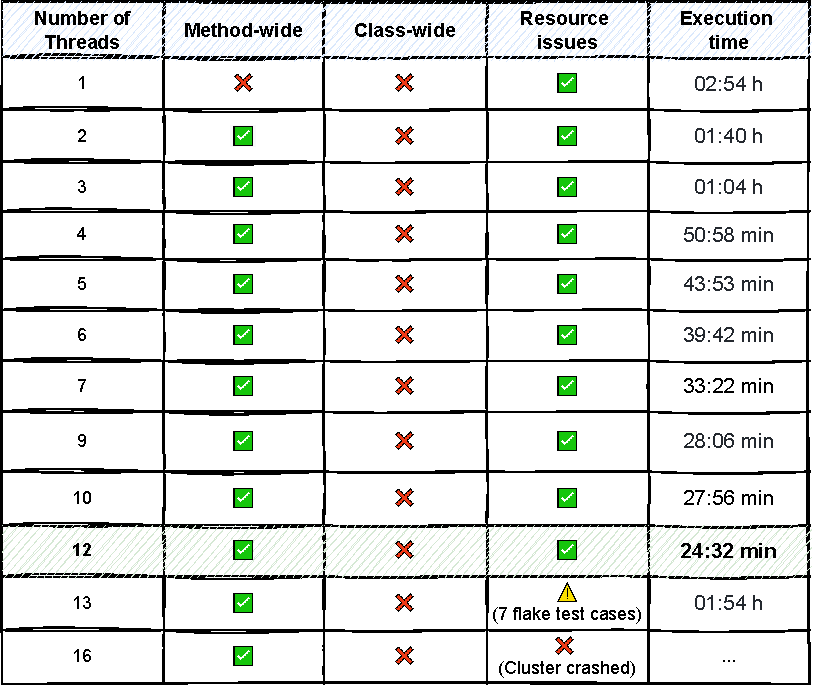
\includegraphics[scale=0.8]{obrazky-figures/08-experiments/preliminary/06-exp-final-smoke-method-wide-ocp}
    \caption{The \textbf{SecurityST} contains twenty-one test cases, and all of them could be executed in parallel
        (i.e., contains @ParallelTest or @ParallelNamespaceTest annotation).
        Moreover, each test case deploys a Kafka cluster, which perfectly verifies if the Kubernetes cluster
        or Minikube (i.e., single-node) can handle such a load.}
    \label{06:tab:01:securityst-ocp-multinode}
\end{table}

\begin{equation}
    \label{eqn:amdalh-limit}
    \lim_{s\to\infty} S_{max} = \frac{1}{1-p} = \frac{1}{1-\frac{171}{174}} = 58x
    \tag{8}
\end{equation}
Our acquired acceleration in a perfect environment is less than $S _{\max} = 58x$ and at the same time $S_{teo} = 17.4x$.
However, this is confirmed by the fact that we will never be better than $S_{\max}$ and also, we will never achieve a
possible theoretical acceleration (i.e., $S_{teo}$) because such results are entirely typical for this kind of experiment.
Overall, our acceleration is $S_{practical} = \frac{174}{24.5} = 7.1x$, which proves following relation $S_{practical} < S_{teo} < S_{\max}$.

%---------------------------------------------------------
%--------------------MINIKUBE PART------------------------
%---------------------------------------------------------

Other preliminary experiments we performed were on more minor instances where it was a matter of course that the results
accelerations compared to a multi-node cluster will be significantly lower and slower.
Therefore, Amdalh's law will also contain a much lower theoretical acceleration.
For a machine containing four virtual cores, the estimated theoretical time is $T_{new\_teo\_medium}$, which is equal to
$T_{new\_teo\_medium} = (1 - \frac{182}{185}) * 185 + \frac{\frac{182}{185}} {4} * 185 = $ approximately 49~minutes.
So the theoretical acceleration of the instance could be $S_{new\_teo\_medium} = \frac{185}{49} = 3.8x$.
Nevertheless, as we can see in Table~\ref{06:tab:01:security-st-minikube}, we did not accomplish such a same acceleration.
However, we have come close enough, and the practical acceleration is $S_{new\_practical\_medium} = \frac{185}{79} = 2.34x$.
We could use a maximum of three cores because, in the case of four cores, the virtual machine crashes due to a lack of memory.
CPU utilisation was approximately 80\% during the use of the four cores.
\begin{table}[ht!]
    \centering
    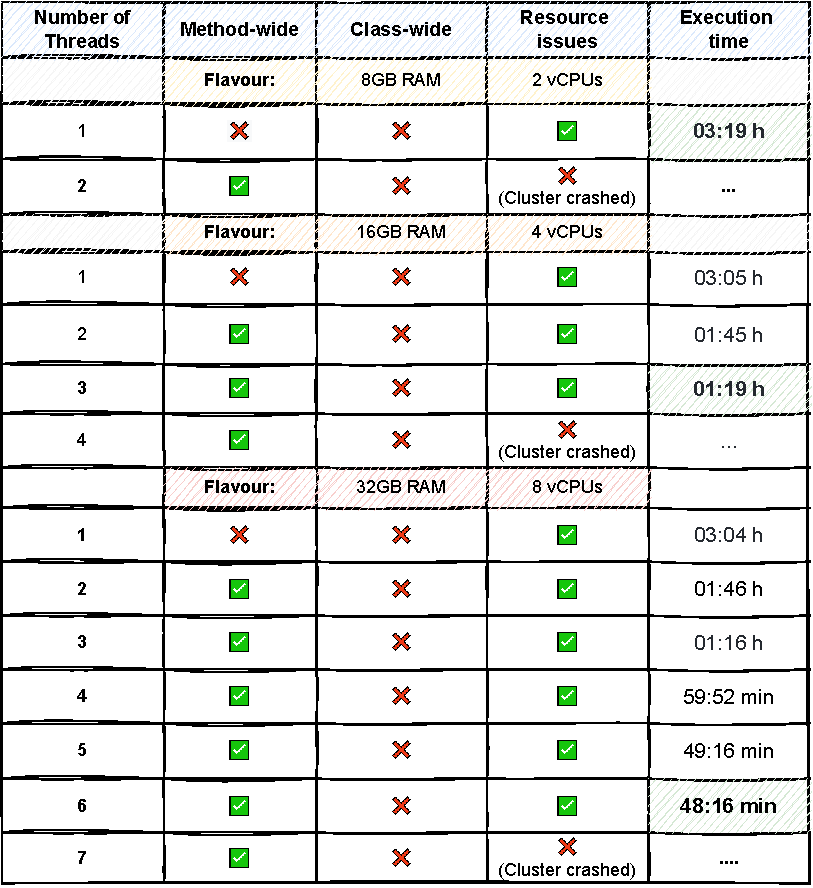
\includegraphics[scale=0.8]{obrazky-figures/08-experiments/preliminary/06-exp-preliminary-minikube-b}
    \caption{Multiple experiments for various flavours of single-node Kubernetes instances for the
    \textbf{SecurityST} suite. Both of these flavours (i.e., orange and red one prove that parallelisation is
    vertically scaling on more minor instances), the yellow one (i.e., using two virtual cores and eight GB RAM)
        is not able to run either two test cases in parallel resulting in OOM problem (i.e., Out of memory).}
    \label{06:tab:01:security-st-minikube}
\end{table}
%-------------------------------------------------------
%-------b) PRELIMINARY EXPERIMENTS FOR CLASS-WIDE-------
%-------------------------------------------------------

We also have done other experiments to prove that our implemented class-wide parallelisation is capable of vertical scaling.
Therefore, we selected a set of test classes that do not need any form of synchronisation or isolation (that is, they do not contain @IsolatedSuite annotation).
Specifically, these will be classes containing the @ParallelSuite annotation, and they are HttpBridgeScramShaST, HttpBridgeTlsST,
ThrottlingQuotaST, TopicST, UserST, ReconciliationST and CruiseControlConfigurationST.
Together they contain thirty test cases where twenty-nine do not need any form of synchronisation, and only one test case needs isolation from other tests.
More precisely, we have ten @ParallelNamespaceTest, for repetition;
these are tests that deploy the Kafka cluster and thus rank among the more resource-intensive.
Next, we have 19 @ParallelTest can also be said to be lightweight variants on the need for total resources, and finally, one @IsolatedTest
guaranteeing isolation from other parallel tests.
In case we would like to calculate a possible theoretical acceleration, it is necessary to know the sequence time and, at the same time, the time of one @IsolatedTest.
The total time of our selected tests is 107~minutes, of which @IsolatedTest lasts two and a half minutes.
If we add the preparation time of the shared Cluster Operator to this, we get to five and a half minutes and therefore, the possible parallel time will be equal to $p = \frac{101.5}{107}$.
The speedup factor is equal to the number of virtual CPUs we have available (i.e., $S = 24$), and thanks to that, all values can be set to
formula as defined above (i.e., Equation~\eqref {eqn:t-new-formula}).
\begin{equation}
    \label{eqn:class-wide-time-ocp}
    T_{new} = (1 - \frac{101.5}{107}) * 107 +  \frac{\frac{101.5}{107}}{24} * 107 =~10~minutes
    \tag{6}
\end{equation}
After the calculation, it turns out that the theoretical acceleration using twenty-four cores will approach ten minutes,
and by this outcome, we can compute theoretical speed up which is $S_{teo} = \frac{T_{old}}{T_{new}} = \frac{107}{10} =~10.7x$
and $\lim_{s\to\infty} S_{\max} = \frac{1}{1-p} = \frac{1}{1-\frac{101.5}{107}} =~19x$.

What should be noted is that for class-wide parallelisation, the best possible scenario is to have a consistent test distribution.
Ideally, such distribution where most test cases support parallel execution and in each test class are enough tests.
(i.e., have test classes containing more minor parallel test cases than configured parallelism).
This gives us the most out of the given type of parallelisation.
For instance, suppose that we have five test classes, and each of them will have two tests (these tests will be capable of parallel execution).
The best possible scenario would be to run such a set of tests with ten threads, guaranteeing that all threads will be busy. However, the test classes generally do not provide such an even distribution, which is almost impossible in practice
(i.e., have the same number of tests for each test class).

\begin{table}[ht!]
    \centering
    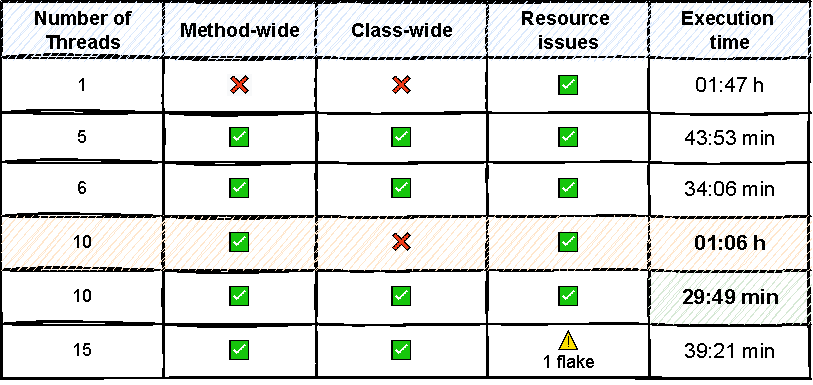
\includegraphics[scale=0.8]{obrazky-figures/08-experiments/preliminary/06-exp-preliminary-cluster-wide-ocp}
    \caption{Experiments aimed at class-wide parallelisation and one execution for method-wide by which we compare these
    two approaches and found non-correlation. Overall thirty test cases were executed (i.e., nineteen @ParallelTest,
        ten @ParallelNamespaceTest and one@IsolatedTest).
    }
    \label{06:tab:01:class-widesecurityst-ocp}
\end{table}

The experiments we performed can be seen in Table~\ref{06:tab:01:class-widesecurityst-ocp} similar to method-wide
we first added a total sequential run to the parallelisation;
then, we increased the number of threads.
Furthermore, we also compared the implementation of method-wide (i.e., orange row colour), where the overall implementation took
significantly more than in the case of class-wide parallelisation (i.e., green row colour).
The main reason why the use of ten threads of class-wide parallelisation was more than half an hour better was because
not more than ten tests were in each test class, and therefore unnecessarily, many threads were used in method-wide parallelisation,
which were not actually used.
On the other hand, class-wide parallelisation has made full use of ten threads, as it can perform several classes simultaneously,
thus significantly increasing the total time.

% HttpBridgeScramShaST - 2 parallel test                  = 2
% HttpBridgeTlsST - 2 parallel test                       = 2
% ThrottlingQuotaST - 4 parallel test                     = 4
% TopicST - 5 parallel test a 1 isolated                  = 6 (1 isolated)
% UserST - 6 parallel test a 2 Paralle namespace test     = 8
% ReconciliationST - 2 parallel namespace test            = 2
% CruiseControlConfigurationST - 6 parallel namespace test= 6
% ----
% 10 PNT, 19 PT a 1 IT

%-------------------------------------------------------------
%------------- END OF PRELIMINARY EXPERIMENTS ----------------
%-------------------------------------------------------------

\section{Production experiments}

In this section, we will include two different experiments.
First, in Section~\ref{06:subsec:acceptance-experiments} they will be described as shown experiments on a small production set of system tests.
Moreover, these experiments provide information on whether parallelisation is applicable even for a small production-based set of tests.
In the next section (i.e., Section~\ref{06:subsec:regression-experiments}), we get a different view of the extensive set
of system tests that are currently available in the Strimzi.

\subsection{Subset of our Strimzi system test}
\label{06:subsec:acceptance-experiments}

This type of experiment will enclose our genuine subset of tests.
These tests also give us whether it is beneficial to perform them parallel.
Since we know that the profile also contains enough test cases for which isolation is necessary (i.e., @IsolatedTest) and test classes (i.e., @IsolatedSuite).
Therefore, a significantly weaker acceleration is expected than the preliminary experiments, which have the best possible parallelisation environment.
Furthermore, since we found out that flavour \emph{2CPUs and 8GB RAM} is not able to perform even two parallel tests, it is thus unnecessary for this type of experiment.

So if we look at a more detailed way in our production-based tests, we find out precisely that it contains 13 test classes and 35 tests.
Of these, 6 test classes require complete isolation (i.e., @IsolatedSuite) and the same for 5 test cases (i.e., @IsolatedTest).
However, what is interesting is to be careful, and parallel tests could sometimes be in border situations taken as @IsolatedTest.
One of the cases is where we have three isolated classes containing only one test that can perform the parallel implementation.
This is because test cases in @IsolatedSuite will only be executed after the calculation is completed by @ParallelSuite or another @IsolatedSuite.
We have eight tests that require complete isolation and 27 tests capable of parallel execution.
However, this fact still does not guarantee that the problem will scale vertically.
One reason is that the \emph{MetricsIsolatedST} test class contains 18 parallel tests, where almost all of them do not last more than a few seconds.
Thus, there will be little success in this class for parallelisation.
At the same time, the overall test set is not an ideal sample for method-wide parallelisation because these are test classes that do not contain
several tests.
However, where it can be a potential success, the use of class-wide parallelisation is not great.
Some paralleled classes (i.e., @ParallelSuite) contain pre-preparation of their test environment (i.e., \emph{HttpBridgeTlsST}, \emph{RollingUpdateST}).
Furthermore, in the case of class-wide parallelisation, they create it independently of the second test class, meaning that where
it will be possible to save time will be mainly in these parts.
However, we do not think we will see an intense acceleration.

% 18x PT, 2x IT...
% ========== SUMMARY ======
% 21x PT, 10PNT (but 3 as iso...), 8x IT
% 8x IT, 6PNT, 21x PT

The experiments we performed on a given test sample do not differ much from the previous ones.
We started with typical sequential execution and gradually increased the number of threads (see Table~\ref{06:tab:02:minikube-accepatance-experiments}).
We found out that during the use of method-wide parallelisation, there was no acceleration at all.
Thus, a scenario where this form of parallelisation is not very suitable due to the small number of tests in the given test classes.
However, where we could potentially succeed was by using class-wide parallelisation.
Within the more powerless machine (i.e., \emph{16GB RAM and four virtual CPUs}), the acceleration was almost non-existent, even in the class-wide case.
\begin{table}[ht!]
    \centering
    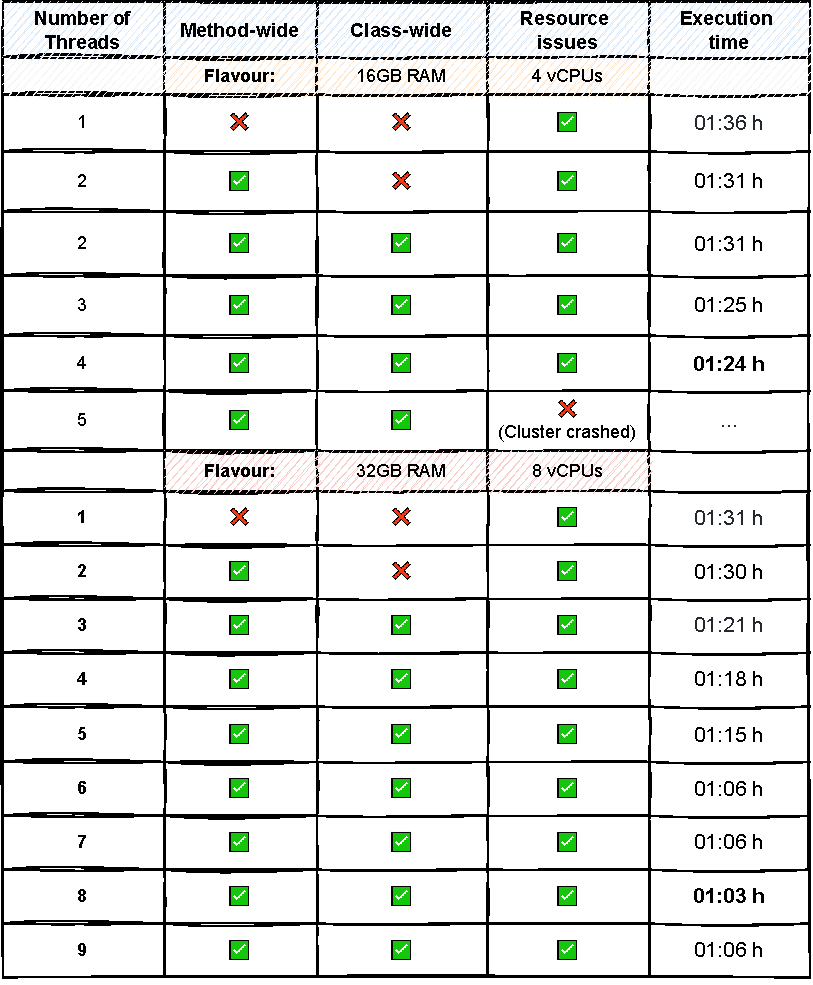
\includegraphics[scale=0.8]{obrazky-figures/08-experiments/acceptance/06-exp-minikube-accpeantace-second}
    \caption{Combination of experiments (i.e., using method and class-wide parallelisation) primarily aiming at class-wide
    parallelisation. Moreover, experiments were performed for more-minor instances of Kubernetes.}
    \label{06:tab:02:minikube-accepatance-experiments}
\end{table}
On the other hand, using a more robust machine (i.e., \emph {32GB RAM and eight virtual CPUs}),
we could get to eight threads with only 1.4x acceleration, which is not very advantageous in using the number of resources needed for parallelisation.
Hence, it is clear that more minor instances of Kubernetes are not suitable for this type of sample (i.e., acceptance production-based) due to the above facts.

At the same time, we wanted to try a similar scenario in the case of using a more significant instance of Kubernetes (i.e., multi-node).
The results we obtained were the same as for the more minor instances of Kubernetes, also due to the size of the test set
(i.e., Table~\ref{06:tab:02:ocp-accepatance-experiments}).
\begin{table}[ht!]
    \centering
    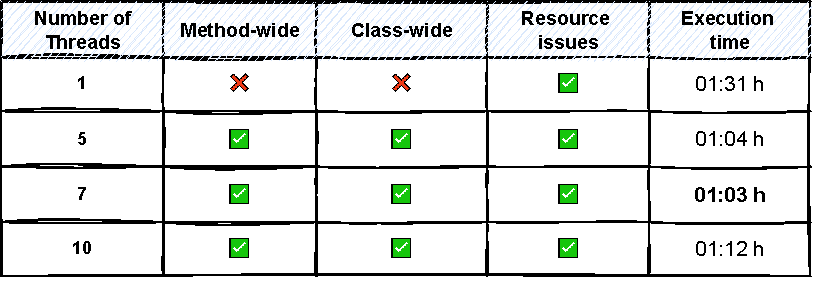
\includegraphics[scale=0.8]{obrazky-figures/08-experiments/acceptance/06-exp-ocp-accpetance-second}
    \caption{Experiments performed by using class-wide parallelisation for a more robust Kubernetes cluster.}
    \label{06:tab:02:ocp-accepatance-experiments}
\end{table}

\subsection{Entire system tests of the Strimzi}
\label{06:subsec:regression-experiments}
% 1. Popísať naše očakávania...
The last type of experiment we tried was a regression (i.e., production\-based).
In other words, a very robust set of test cases contains everything (i.e., @IsolatedTest, @IsolatedSuite,
@ParallelTest, @ParallelSuite).
Currently, this test sample contains approximately 65 test classes, and more than half of them are classes
requiring synchronisation (i.e., @IsolatedSuite).
Specifically, these are 37 isolated classes, and with the use of the add-on, we find that there are classes that
can perform them at the same time precisely 28.
This quantification can give us an approximate possible result of the experiments.
Given that sequential execution takes almost twenty-one hours, the ideal scenario would be to get below half
(i.e., ten hours) of execution time.
A total of four types of experiments will be performed; (a) VM with 16GB RAM and four virtual cores,
(b) VM with 32GB RAM and eight virtual cores, (c) Kubernetes cluster with six nodes (three masters and three workers)
and (d) Kubernetes cluster with nine nodes (three masters and six workers).
We do not expect much acceleration for (a) because this is a test suite when OOM may have a problem.
This is mainly due to test cases containing the component \emph{KafkaMirrorMaker} or \emph{KafkaMirrorMaker2}, which
needs a lot of RAM. On the other hand, for alternative (b), we already assume an acceleration approaching half.
At the same time, however, it will perform method-wide parallelisation for both types of experiments.
In another Kubernetes instance (c) type, we assume the possible implementation of at least five threads
in parallel and, thus, some acceleration.
Finally, for (d), it is a matter of course that the most significant possible acceleration is expected and,
at the same time, the use of class-wide parallelisation for a vast number of threads.

% 2. Popísať výsledky
In the first run of experiments for small instances of Kubernetes (i.e., using one VM), we obtained the following information.
For VMs with 16GB RAM and four virtual cores, no form of parallelisation is possible because already with method-wide parallelisations
with the use of two threads, the given VM falls on the lack of memory (Table~\ref{06:tab:02:minikube-regression-experiments}).
\begin{table}[ht!]
    \centering
    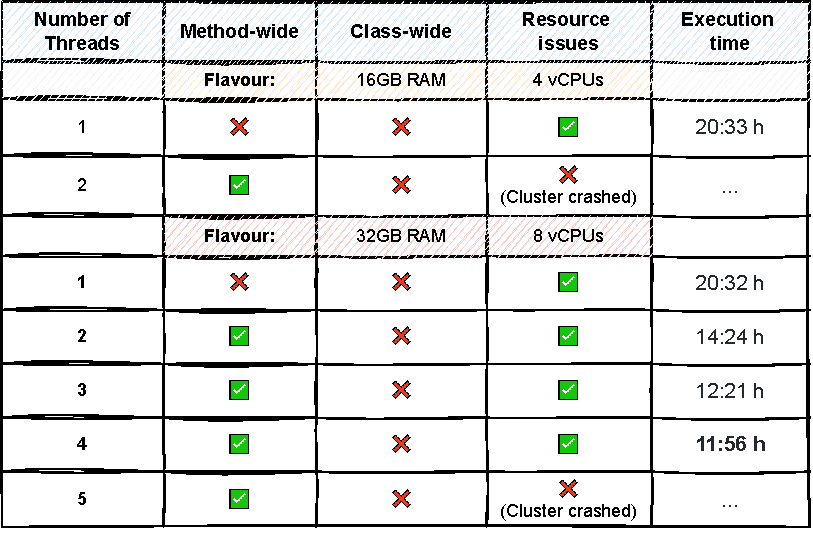
\includegraphics[scale=0.8]{obrazky-figures/08-experiments/regression/06-minikube-regression}
    \caption{Combination of experiments (i.e., using method parallelisation) on production-based test sample with different VMs.}
    \label{06:tab:02:minikube-regression-experiments}
\end{table}
This is the case in test cases using the \emph{KafkaMirrorMaker} or \emph{KafkaMirrorMaker2} components.
At the same time, the combination of \emph{KafkaConnect} with \emph{KafkaMirrorMaker/2}.
Let us remember that one component of \emph {KafkaMirrorMaker/2} requires two Kafka clusters, and hence
is very memory intensive.

The second type of experiment using a more powerful VM was slightly more favourable in terms of results.
We could even use four threads where the total time spent performing was 12h from the flood 21h.
However, using five threads, we got into the same problem as in previous experiments (i.e., OOM problem), as
shown in Table~\ref{06:tab:02:minikube-regression-experiments}.
Overall, it can be assessed (for small instances of Kubernetes) that ideal candidates for this test sample
will use VM with 32GB RAM and eight virtual cores.

Another form of experimentation (i.e., (c) and (d)) they were even more massive on resources.
Therefore, we expected better results.
\begin{table}[ht!]
    \centering
    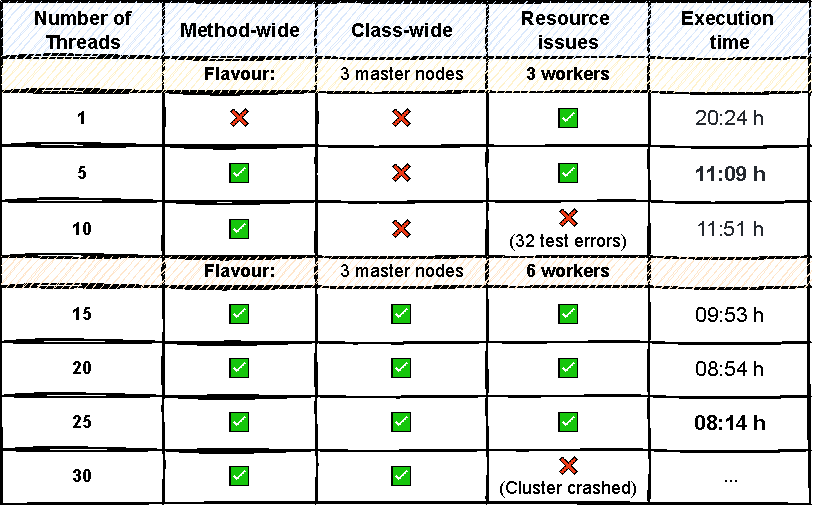
\includegraphics[scale=0.8]{obrazky-figures/08-experiments/regression/06-exp-ocp-regression}
    \caption{Experiments performed by using method-wide and class-wide parallelisation for a more robust Kubernetes
    clusters (variation with three and six worker nodes).}
    \label{06:tab:02:ocp-regression-experiments}
\end{table}
For the Kubernetes cluster using three master and three worker nodes, we got the best results using five threads and were
we can get from 21h to 11h, as can be seen in Table~\ref{06:tab:02:ocp-regression-experiments}.
When we used more threads, the result was worse, or the test cases fell due to a lack of memory (e.g, using
ten threads, we got 32 error tests).

The results were much better for the Kubernetes cluster using three master and six worker nodes.
We could use up to twenty-five threads, which resulted in a decrease in computing time.
Interestingly, almost half of the test classes that support class-wide parallelization (i.e., @ParallelSuites)
improved its total exercise time from about eight hours to one hour, which results in up to 8-fold acceleration.
On the other hand, we could not fully use the strength within the remaining thirty-seven test classes that need an isolation environment (i.e., @IsolatedSuite).
It is evident that tests are performed in parallel in a given class, but occasionally there are five or fewer tests in a given class, which
prolongs the entire execution time.
From the sequential execution time (i.e., twenty-one hours), we got to eight hours (Table~\ref{06:tab:02:ocp-regression-experiments}).
Moreover, one hypothesis would undoubtedly improve the overall performance, but it would also worsen the overall readability of the test sample.
For instance, if we were to re-structure the test suites, where we would be test classes (mainly @IsolatedSuite).
Then we add test cases that require the same \emph{Cluster Operator} configuration, and these test suites would contain a maximum of twenty-five test cases.
It would significantly improve overall time because test classes will not contain less than five test cases, resulting in a situation where most threads are working.
Therefore, we eliminate scenarios where we configure twenty-five threads running in parallel, and some test classes have only three or fewer test cases, meaning that the seventeenth threads are sleeping.
Re-structuring our test classes can be very friendly at first glance.
Unfortunately, we would sacrifice readability (e.g., tests that should belong to a separate test class we combine into some most similar), thus reducing scenarios where we can have @IsolatedSuite with less than five test cases.
Nevertheless, we could end up in a scenario where these test cases in one @IsolatedSuite will not have any standard features.
From a performance point of view, this can also be summarized by the following quote said by Donald Ervin Knuth.
\begin{quote}
    \textit{Premature optimization is the root of all evil (or at least most of it) in programming.}
\end{quote}

In the case of using 30 threads, we got to the problem of OOM and Kubernetes cluster crashing.
We can evaluate that Kubernetes for a given test sample is the optimal candidate
cluster using three master and six workers nodes for larger instances.

\chapter{Conclusion}
\label{08:chapter:title}

The thesis began with a description of the basic principles of \emph{Kubernetes} and \emph{Kafka}.
Furthermore, we described a project that encapsulates Kafka and uses it on top of the Kubernetes (i.e., Strimzi).
We further explained the architecture and principles in the system tests of the Strimzi project.
In addition, we gained knowledge about parallel execution, which we successfully used in this thesis.
Moreover, we identified the challenges of the current system test architecture.
Therefore, we designed and implemented a solution to solve these problems (i.e., using multiple pipelines and creating sub-sets of
tests is not horizontally scalable due to our cloud services that provide resources).
Thus, this information motivated us to design and implement a mechanism of fine-grained parallelism in our test framework (i.e., using memory and central processing units) that the cloud services offer us.
Finally, our experiments showed that parallelisation could scale vertically for different test samples.

Based on the performed experiments, we found that within the environment that fully supports parallelisation, there were results
the acceleration within factor 8.
We obtained the identical factor in the case of production experiments (i.e., from eight to one hour) when performing only classes that support class-wide parallelisation (i.e., @ParallelSuite).
By contrast, overall production experiments (i.e., together with @IsolatedSuite) showed partially more inadequate results (i.e., a factor of 2.5).
We reach such a factor mainly due to the structure of the test classes and their content (i.e., the number of tests within the test class; meaning a @IsolatedSuite with fewer than five test cases when twenty-five threads in parallel are configured and thus twenty threads sleep).
Furthermore, more than half of the classes require to perform in complete isolation (i.e., @IsolatedSuite).

We contributed the given code to the open-sourced project Strimzi, available on
Github\footnote{Strimzi Github repository \---\ \url{https://github.com/strimzi/strimzi-kafka-operator}},
which also makes it viable to inspire other \emph{kube-native} products to enforce such solutions.
Making parallel execution possible started from 0.23.0 (released in May 2021) to the 0.29.0 Strimzi version.
Whether a method or class-wide parallelisation, both steps have been completed and merged into the main branch of
the Strimzi project, where this implementation will be available from version 0.29.0.
Our parallelism model of system tests is used in continuous integration systems (i.e., Jenkins, Azure Pipelines), where the overall computational time is much faster than in sequential computational computation (proved by experiments).